\documentclass{standalone}
\usepackage{tikz}
\usetikzlibrary{patterns, positioning}

\begin{document}
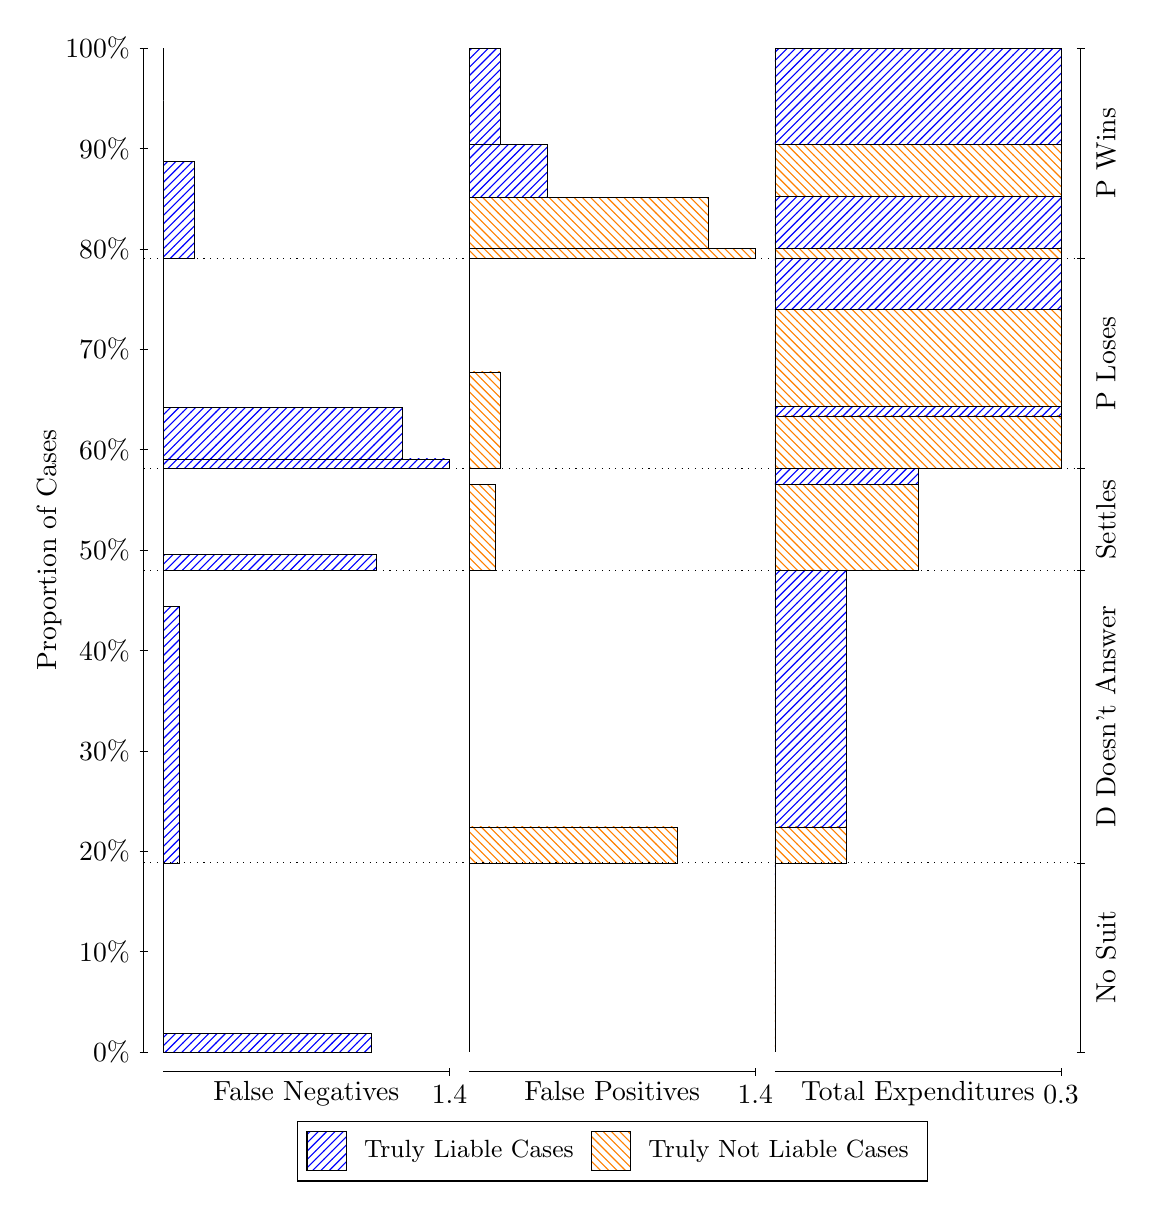
\begin{tikzpicture}
\draw[black, very thin] (1.5,1.75) -- (1.5,14.5);
\node[rotate=90, anchor=center] at (0.3, 8.125) {Proportion of Cases};
\draw[black, very thin] (1.45,1.75) -- (1.55,1.75);
\node[anchor=east] at (1.45, 1.75) {0\%};
\draw[black, very thin] (1.45,3.025) -- (1.55,3.025);
\node[anchor=east] at (1.45, 3.025) {10\%};
\draw[black, very thin] (1.45,4.3) -- (1.55,4.3);
\node[anchor=east] at (1.45, 4.3) {20\%};
\draw[black, very thin] (1.45,5.575) -- (1.55,5.575);
\node[anchor=east] at (1.45, 5.575) {30\%};
\draw[black, very thin] (1.45,6.85) -- (1.55,6.85);
\node[anchor=east] at (1.45, 6.85) {40\%};
\draw[black, very thin] (1.45,8.125) -- (1.55,8.125);
\node[anchor=east] at (1.45, 8.125) {50\%};
\draw[black, very thin] (1.45,9.4) -- (1.55,9.4);
\node[anchor=east] at (1.45, 9.4) {60\%};
\draw[black, very thin] (1.45,10.675) -- (1.55,10.675);
\node[anchor=east] at (1.45, 10.675) {70\%};
\draw[black, very thin] (1.45,11.95) -- (1.55,11.95);
\node[anchor=east] at (1.45, 11.95) {80\%};
\draw[black, very thin] (1.45,13.225) -- (1.55,13.225);
\node[anchor=east] at (1.45, 13.225) {90\%};
\draw[black, very thin] (1.45,14.5) -- (1.55,14.5);
\node[anchor=east] at (1.45, 14.5) {100\%};

\draw[black, very thin] (13.4,1.75) -- (13.4,14.5);
\draw[black, very thin] (13.35,1.75) -- (13.45,1.75);
\node[anchor=west] at (13.35, 1.75) {};
\draw[black, very thin] (13.35,4.1507) -- (13.45,4.1507);
\node[anchor=west] at (13.35, 4.1507) {};
\draw[black, very thin] (13.35,7.8663) -- (13.45,7.8663);
\node[anchor=west] at (13.35, 7.8663) {};
\draw[black, very thin] (13.35,9.1605) -- (13.45,9.1605);
\node[anchor=west] at (13.35, 9.1605) {};
\draw[black, very thin] (13.35,11.83) -- (13.45,11.83);
\node[anchor=west] at (13.35, 11.83) {};
\draw[black, very thin] (13.35,14.5) -- (13.45,14.5);
\node[anchor=west] at (13.35, 14.5) {};

\draw[black, very thin, pattern color=blue, pattern=north east lines] (1.75,1.75) rectangle (4.3924,1.991);
\draw[black, very thin, pattern color=orange, pattern=north west lines] (1.75,1.991) rectangle (1.75,4.1507);
\draw[black, very thin, pattern color=blue, pattern=north east lines] (1.75,4.1507) rectangle (1.9482,7.4086);
\draw[black, very thin, pattern color=orange, pattern=north west lines] (1.75,7.4086) rectangle (1.75,7.8663);
\draw[black, very thin, pattern color=blue, pattern=north east lines] (1.75,7.8663) rectangle (4.4585,8.0725);
\draw[black, very thin, pattern color=orange, pattern=north west lines] (1.75,8.0725) rectangle (1.75,9.1605);
\draw[black, very thin, pattern color=blue, pattern=north east lines] (1.75,9.1605) rectangle (5.3833,9.2814);
\draw[black, very thin, pattern color=blue, pattern=north east lines] (1.75,9.2814) rectangle (4.7888,9.9348);
\draw[black, very thin, pattern color=orange, pattern=north west lines] (1.75,9.9348) rectangle (1.75,11.83);
\draw[black, very thin, pattern color=blue, pattern=north east lines] (1.75,11.83) rectangle (2.1464,13.057);
\draw[black, very thin, pattern color=orange, pattern=north west lines] (1.75,13.057) rectangle (1.75,13.832);
\draw[black, very thin, pattern color=blue, pattern=north east lines] (1.75,13.832) rectangle (1.75,14.5);
\draw[black, very thin, pattern color=orange, pattern=north west lines] (5.6333,1.75) rectangle (5.6333,3.9097);
\draw[black, very thin, pattern color=blue, pattern=north east lines] (5.6333,3.9097) rectangle (5.6333,4.1507);
\draw[black, very thin, pattern color=orange, pattern=north west lines] (5.6333,4.1507) rectangle (8.2758,4.6084);
\draw[black, very thin, pattern color=blue, pattern=north east lines] (5.6333,4.6084) rectangle (5.6333,7.8663);
\draw[black, very thin, pattern color=orange, pattern=north west lines] (5.6333,7.8663) rectangle (5.9636,8.9543);
\draw[black, very thin, pattern color=blue, pattern=north east lines] (5.6333,8.9543) rectangle (5.6333,9.1605);
\draw[black, very thin, pattern color=orange, pattern=north west lines] (5.6333,9.1605) rectangle (6.0297,10.388);
\draw[black, very thin, pattern color=orange, pattern=north west lines] (5.6333,10.388) rectangle (5.6333,11.056);
\draw[black, very thin, pattern color=blue, pattern=north east lines] (5.6333,11.056) rectangle (5.6333,11.83);
\draw[black, very thin, pattern color=orange, pattern=north west lines] (5.6333,11.83) rectangle (9.2667,11.951);
\draw[black, very thin, pattern color=orange, pattern=north west lines] (5.6333,11.951) rectangle (8.6721,12.605);
\draw[black, very thin, pattern color=blue, pattern=north east lines] (5.6333,12.605) rectangle (6.6242,13.273);
\draw[black, very thin, pattern color=blue, pattern=north east lines] (5.6333,13.273) rectangle (6.0297,14.5);
\draw[black, very thin, pattern color=orange, pattern=north west lines] (9.5167,1.75) rectangle (9.5167,3.9097);
\draw[black, very thin, pattern color=blue, pattern=north east lines] (9.5167,3.9097) rectangle (9.5167,4.1507);
\draw[black, very thin, pattern color=orange, pattern=north west lines] (9.5167,4.1507) rectangle (10.425,4.6084);
\draw[black, very thin, pattern color=blue, pattern=north east lines] (9.5167,4.6084) rectangle (10.425,7.8663);
\draw[black, very thin, pattern color=orange, pattern=north west lines] (9.5167,7.8663) rectangle (11.333,8.9543);
\draw[black, very thin, pattern color=blue, pattern=north east lines] (9.5167,8.9543) rectangle (11.333,9.1605);
\draw[black, very thin, pattern color=orange, pattern=north west lines] (9.5167,9.1605) rectangle (13.15,9.8288);
\draw[black, very thin, pattern color=blue, pattern=north east lines] (9.5167,9.8288) rectangle (13.15,9.9497);
\draw[black, very thin, pattern color=orange, pattern=north west lines] (9.5167,9.9497) rectangle (13.15,11.177);
\draw[black, very thin, pattern color=blue, pattern=north east lines] (9.5167,11.177) rectangle (13.15,11.83);
\draw[black, very thin, pattern color=orange, pattern=north west lines] (9.5167,11.83) rectangle (13.15,11.951);
\draw[black, very thin, pattern color=blue, pattern=north east lines] (9.5167,11.951) rectangle (13.15,12.619);
\draw[black, very thin, pattern color=orange, pattern=north west lines] (9.5167,12.619) rectangle (13.15,13.273);
\draw[black, very thin, pattern color=blue, pattern=north east lines] (9.5167,13.273) rectangle (13.15,14.5);
\draw[black, dotted] (1.5,4.1507) -- (13.4,4.1507);
\draw[black, dotted] (1.5,7.8663) -- (13.4,7.8663);
\draw[black, dotted] (1.5,9.1605) -- (13.4,9.1605);
\draw[black, dotted] (1.5,11.83) -- (13.4,11.83);
\draw[black, very thin] (1.75,1.5) -- (5.3833,1.5);
\node[anchor=north] at (3.5667, 1.5) {False Negatives};
\draw[black, very thin] (5.3833,1.45) -- (5.3833,1.55);
\node[anchor=north] at (5.3833, 1.45) {1.4};

\draw[black, very thin] (5.6333,1.5) -- (9.2667,1.5);
\node[anchor=north] at (7.45, 1.5) {False Positives};
\draw[black, very thin] (9.2667,1.45) -- (9.2667,1.55);
\node[anchor=north] at (9.2667, 1.45) {1.4};

\draw[black, very thin] (9.5167,1.5) -- (13.15,1.5);
\node[anchor=north] at (11.333, 1.5) {Total Expenditures};
\draw[black, very thin] (13.15,1.45) -- (13.15,1.55);
\node[anchor=north] at (13.15, 1.45) {0.3};

\node[black, centered, rotate=90] at (13.72, 2.9503) {No Suit};
\node[black, centered, rotate=90] at (13.72, 6.0085) {D Doesn't Answer};
\node[black, centered, rotate=90] at (13.72, 8.5134) {Settles};
\node[black, centered, rotate=90] at (13.72, 10.495) {P Loses};
\node[black, centered, rotate=90] at (13.72, 13.165) {P Wins};

\draw (7.449999999999999,1.5) node[draw=none] (baseCoordinate) {};
\begin{scope}[align=center]
        \matrix[scale=0.5, draw=black, below=0.5cm of baseCoordinate, nodes={draw}, column sep=0.1cm]{
            \node[rectangle, draw, minimum width=0.5cm, minimum height=0.5cm, pattern=north east lines, pattern color=blue] {}; &
            \node[draw=none, font=\small] (B) {Truly Liable Cases}; &
            \node[rectangle, draw, minimum width=0.5cm, minimum height=0.5cm, pattern=north west lines, pattern color=orange] {}; &
            \node[draw=none, font=\small] (B) {Truly Not Liable Cases}; \\
            };
\end{scope}

\end{tikzpicture}
\end{document}